\documentclass{article}
\usepackage{pgfplots}
\usepackage{tikz}
\usepackage{amsmath}
\pgfplotsset{compat=1.18}

\begin{document}

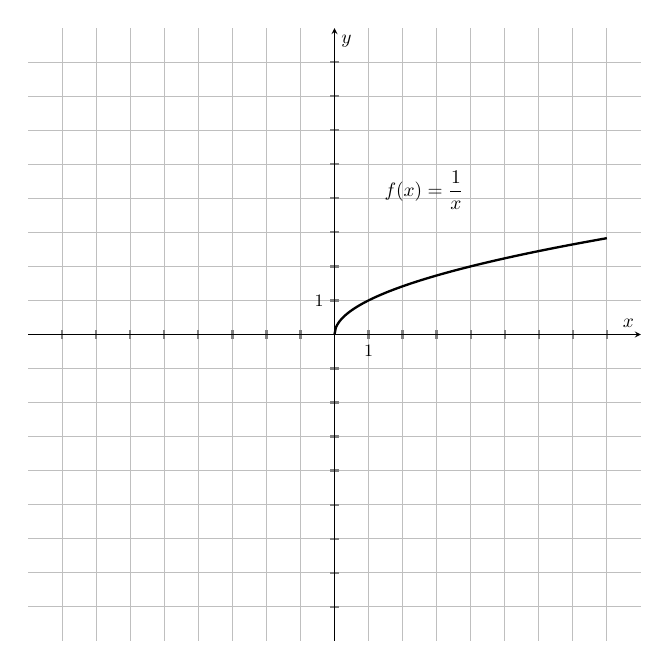
\begin{tikzpicture}[scale=0.7]
\begin{axis}[
  axis lines=center,
  grid=major,
  width=5in,
  height=5in,
  xmin=-8,
  xmax=8,
  ymin=-8,
  ymax=8,
  xlabel={$x$},
  ylabel={$y$},
  enlargelimits={abs=1},
  xtick={-8,-7,...,8},
  ytick={-8,-7,...,8},
  xticklabels={,,,,,,,,0,1,,,,,,,},
  yticklabels={,,,,,,,,,1,,,,,,,},
  xlabel style={at={(rel axis cs:1,0.5)}},
  ylabel style={at={(rel axis cs:0.5,1)}},
  tick style={very thick},
  ticklabel style={font=\small},
  legend style={
    at={(rel axis cs:1,1)},
    anchor=north west,
    draw=none,
    inner sep=0pt,
    fill=gray!10}
]

\addplot [very thick, domain=0:8, samples=200] {x^(0.5)};
\node[below left] at (axis cs:4,5) {$f(x)=\dfrac{1}{x}$};
\end{axis}
\end{tikzpicture}

\end{document}

